\documentclass[a4paper, 12pt]{report}		% general format

%%%% Charset
\usepackage{cmap}							% make PDF files searchable and copyable
\usepackage[utf8]{inputenc}					% accept different input encodings
\usepackage[T2A]{fontenc}					% russian font
\usepackage[russian]{babel}					% multilingual support (T2A)

%%%% Graphics
\usepackage[dvipsnames]{xcolor}			% driver-independent color extensions
\usepackage{graphicx}						% enhanced support for graphics
\usepackage{wrapfig}						% produces figures which text can flow around

%%%% Math
\usepackage{amsmath}						% American Mathematical Society (AMS) math facilities
\usepackage{amsfonts}						% fonts from the AMS
\usepackage{amssymb}						% additional math symbols

%%%% Typograpy (don't forget about cm-super)
\usepackage{microtype}						% subliminal refinements towards typographical perfection
\linespread{1.3}							% line spacing
\usepackage[left=2.5cm, right=1.5cm, top=2.5cm, bottom=2.5cm]{geometry}
\setlength{\parindent}{0pt}					% we don't want any paragraph indentation
\renewcommand{\chaptername}{}

%%%% Other
\usepackage{url}							% verbatim with URL-sensitive line breaks
%\DeclareUnicodeCharacter{00A0}{~}

%------------------------------------------------------------------------------
\usepackage{listings}						% typeset source code listings

% Цвета для кода
\definecolor{string}{HTML}{101AF9}			% цвет строк в коде
\definecolor{comment}{HTML}{3F7F5F}		% цвет комментариев в коде
\definecolor{keyword}{HTML}{5F1441}		% цвет ключевых слов в коде
\definecolor{morecomment}{HTML}{8000FF}	% цвет include и других элементов в коде
\definecolor{captiontext}{HTML}{FFFFFF}	% цвет текста заголовка в коде
\definecolor{captionbk}{HTML}{999999}		% цвет фона заголовка в коде
\definecolor{bk}{HTML}{FFFFFF}				% цвет фона в коде
\definecolor{frame}{HTML}{999999}			% цвет рамки в коде

% Настройки отображения кода
\lstset{
	language=C++,							% Язык кода по умолчанию
	morekeywords={*,...},					% если хотите добавить ключевые слова, то добавляйте
	% Цвета
	keywordstyle=\color{keyword}\ttfamily\bfseries,
	stringstyle=\color{string}\ttfamily,
	commentstyle=\color{comment}\ttfamily\itshape,
	morecomment=[l][\color{morecomment}]{\#},
	% Настройки отображения
	breaklines=true,						% Перенос длинных строк
	basicstyle=\ttfamily\footnotesize,		% Шрифт для отображения кода
	backgroundcolor=\color{bk},				% Цвет фона кода
	%frame=lrb,xleftmargin=\fboxsep,xrightmargin=-\fboxsep, % Рамка, подогнанная к заголовку
	frame=tblr								% draw a frame at all sides of the code block
	rulecolor=\color{frame},				% Цвет рамки
	tabsize=2,								% tab space width
	showstringspaces=false,					% don't mark spaces in strings
	% Настройка отображения номеров строк. Если не нужно, то удалите весь блок
	numbers=left,							% Слева отображаются номера строк
	stepnumber=1,							% Каждую строку нумеровать
	numbersep=5pt,							% Отступ от кода
	numberstyle=\small\color{black},		% Стиль написания номеров строк
	% Для отображения русского языка
	extendedchars=true,
	literate={Ö}{{\"O}}1
	 	{Ä}{{\"A}}1
	 	{Ü}{{\"U}}1
		{ß}{{\ss}}1
		{ü}{{\"u}}1
		{ä}{{\"a}}1
		{ö}{{\"o}}1
		{~}{{\textasciitilde}}1
		{а}{{\selectfont\char224}}1
		{б}{{\selectfont\char225}}1
		{в}{{\selectfont\char226}}1
		{г}{{\selectfont\char227}}1
		{д}{{\selectfont\char228}}1
		{е}{{\selectfont\char229}}1
		{ё}{{\"e}}1
		{ж}{{\selectfont\char230}}1
		{з}{{\selectfont\char231}}1
		{и}{{\selectfont\char232}}1
		{й}{{\selectfont\char233}}1
		{к}{{\selectfont\char234}}1
		{л}{{\selectfont\char235}}1
		{м}{{\selectfont\char236}}1
		{н}{{\selectfont\char237}}1
		{о}{{\selectfont\char238}}1
		{п}{{\selectfont\char239}}1
		{р}{{\selectfont\char240}}1
		{с}{{\selectfont\char241}}1
		{т}{{\selectfont\char242}}1
		{у}{{\selectfont\char243}}1
		{ф}{{\selectfont\char244}}1
		{х}{{\selectfont\char245}}1
		{ц}{{\selectfont\char246}}1
		{ч}{{\selectfont\char247}}1
		{ш}{{\selectfont\char248}}1
		{щ}{{\selectfont\char249}}1
		{ъ}{{\selectfont\char250}}1
		{ы}{{\selectfont\char251}}1
		{ь}{{\selectfont\char252}}1
		{э}{{\selectfont\char253}}1
		{ю}{{\selectfont\char254}}1
		{я}{{\selectfont\char255}}1
		{А}{{\selectfont\char192}}1
		{Б}{{\selectfont\char193}}1
		{В}{{\selectfont\char194}}1
		{Г}{{\selectfont\char195}}1
		{Д}{{\selectfont\char196}}1
		{Е}{{\selectfont\char197}}1
		{Ё}{{\"E}}1
		{Ж}{{\selectfont\char198}}1
		{З}{{\selectfont\char199}}1
		{И}{{\selectfont\char200}}1
		{Й}{{\selectfont\char201}}1
		{К}{{\selectfont\char202}}1
		{Л}{{\selectfont\char203}}1
		{М}{{\selectfont\char204}}1
		{Н}{{\selectfont\char205}}1
		{О}{{\selectfont\char206}}1
		{П}{{\selectfont\char207}}1
		{Р}{{\selectfont\char208}}1
		{С}{{\selectfont\char209}}1
		{Т}{{\selectfont\char210}}1
		{У}{{\selectfont\char211}}1
		{Ф}{{\selectfont\char212}}1
		{Х}{{\selectfont\char213}}1
		{Ц}{{\selectfont\char214}}1
		{Ч}{{\selectfont\char215}}1
		{Ш}{{\selectfont\char216}}1
		{Щ}{{\selectfont\char217}}1
		{Ъ}{{\selectfont\char218}}1
		{Ы}{{\selectfont\char219}}1
		{Ь}{{\selectfont\char220}}1
		{Э}{{\selectfont\char221}}1
		{Ю}{{\selectfont\char222}}1
		{Я}{{\selectfont\char223}}1
		{і}{{\selectfont\char105}}1
		{ї}{{\selectfont\char168}}1
		{є}{{\selectfont\char185}}1
		{ґ}{{\selectfont\char160}}1
		{І}{{\selectfont\char73}}1
		{Ї}{{\selectfont\char136}}1
		{Є}{{\selectfont\char153}}1
		{Ґ}{{\selectfont\char128}}1
}

% Для настройки заголовка кода
\usepackage{caption}
\DeclareCaptionFont{white}{\color{сaptiontext}}
\DeclareCaptionFormat{listing}{\parbox{\linewidth}{\colorbox{сaptionbk}{\parbox{\linewidth}{#1#2#3}}\vskip-4pt}}
%\captionsetup[lstlisting]{format=listing,labelfont=white,textfont=white}
\renewcommand{\lstlistingname}{Листинг} % Переименование Listings в нужное именование структуры

%------------------------------------------------------------------------------
\begin{document}

\begin{titlepage}
\thispagestyle{empty}

\begin{center}
Санкт-Петербургский государственный политехнический университет \\
Институт Информационных Технологий и Управления \\*
Кафедра компьютерных систем и программных технологий \\*
\hrulefill
\end{center}

\vspace{18em}

\begin{center}
\Large Отчёт по расчётной работе № 2 \\ по предмету «Системное программное обеспечение» \\
\end{center}

\vspace{1em}

% \linebreak
\begin{center}
\textsc{\textbf{Межпроцессное взаимодействие в ОС Windows}}
\end{center}

\vspace{16em}

\begin{flushleft}
Работу выполнил студент гр. 53501/3\hrulefill Мартынов С. А. \\
\vspace{1.5em}
Работу принял преподаватель \hrulefill Душутина Е. В. \\
\end{flushleft}

\vspace{\fill}

\begin{center}
Санкт-Петербург \\
2014
\end{center}

\end{titlepage}
%------------------------------------------------
\setcounter{page}{2}
\tableofcontents
%------------------------------------------------

\chapter*{Постановка задачи}
\addcontentsline{toc}{chapter}{Постановка задачи}

В рамках данной работы необходимо ознакомиться с основными механизмами межпроцессное взаимодействие в ОС Windows
\begin{enumerate}
    \item Анонимные каналы;
    \item Именованные каналы \\
        (локальная/сетевая реализация);
    \item Почтовые ящики;
    \item Shared memory;
    \item Сокеты;
    \item Порты завершения;
    \item Сигналы.
\end{enumerate}

В процессе изучения предполагается разработать простой (консольный) мгновенный обмен сообщениями.

%------------------------------------------------
\chapter*{Введение}
\addcontentsline{toc}{chapter}{Введение}

\vspace{1em}
Для тестирования сетевых реализаций используются два виртуальные машины (Win7) под управлением гипервизора VirtualBox. Сетевое подключение осуществляется в режиме bridge. Топология представлена на рисунке 1. Разницы между виртуальной и физической средой быть не должно.

\begin{figure}[h!]
\centering
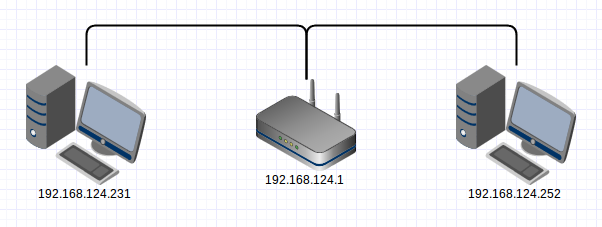
\includegraphics[scale=0.7]{res/01_topology}
\caption{Топология сети.}
\end{figure}

\vspace{1em}
Все результаты, представленные в данном отчёте получены с использованием Microsoft Windows 7 Ultimate Service Pack 1 64-bit (build 7601). Для разработки использовалась Microsoft Visual Studio Express 2013 for Windows Desktops (Version 12.0.30723.00 Update 3). В качестве отладчика использовался Microsoft WinDbg (release 6.3.9600.16384).

Для логирования использовался код, приведённый в листинге 1. Этот файл подключается в первых строках каждого проекта. Он создаёт файл, с именем идентичным исполняемой программе, и записывает туда все события.

\lstinputlisting[language=C++, caption={Логер, используемый во всех проектах}]
{../../src/InterProcessCommunication/AnonymousPipeServer/logger.h}

\vspace{1em}
Исходный код всех представленных листингов доступен по адресу \\ \url{https://github.com/SemenMartynov/SPbPU_SystemProgramming}.

%------------------------------------------------
\chapter*{Анонимные каналы}
\addcontentsline{toc}{chapter}{Анонимные каналы}

Анонимные каналы (anonymous channels) Windows обеспечивают однонаправленное (полудуплексное) посимвольное межпроцессное взаимодействие. Каждый канал имеет два дескриптора: дескриптор чтения (read handle) и дескриптор записи (write handle). Функция, с помощью которой создаются анонимные каналы, имеет следующий прототип:

\begin{verbatim}
BOOL CreatePipe(PHANDLE phRead, PHANDLE phWrite,
                                  LPSECURITY_ATTRIBUTES lpsa, DWORD cbPipe)
\end{verbatim}

Дескрипторы каналов часто бывают наследуемыми; причины этого станут понятными из приведенного ниже примера. Значение параметра cbPipe, указывающее размер канала в байтах, носит рекомендательный характер, причем значению 0 соответствует размер канала по умолчанию.

Чтобы канал можно было использовать для IPC, должен существовать еще один процесс, и для этого процесса требуется один из дескрипторов канала. Предположим, например, что родительскому процессу, вызвавшему функцию CreatePipe, необходимо вывести данные, которые нужны дочернему процессу. Тогда возникает вопрос о том, как передать дочернему процессу дескриптор чтения (phRead). Родительский процесс осуществляет это, устанавливая дескриптор стандартного ввода в структуре STARTUPINFO для дочерней процедуры равным *phRead.

Чтение с использованием дескриптора чтения канала блокируется, если канал пуст. В противном случае в процессе чтения будет воспринято столько байтов, сколько имеется в канале, вплоть до количества, указанного при вызове функции ReadFile. Операция записи в заполненный канал, которая выполняется с использованием буфера в памяти, также будет блокирована.

Наконец, анонимные каналы обеспечивают только однонаправленное взаимодействие. Для двухстороннего взаимодействия необходимы два канала.

В листинге 2 и 3 демонстрируются серверный и клиентский модуль программы, в которой используется передача дескрипторов через наследование. Анонимный канал является полудуплексным, поэтому для организации эхо-сервера было необходимо создавать 2 канала (для передачи от клиента к серверу и в обратном направлении). При этом ненужные дескрипторы каналов закрываются только на стороне сервера (т.к. клиент наследует 4 дескриптора, а явно передаются только 2). Дескрипторы каналов связываются со стандартным вводом и выводом клиентского процесса. Для вывода информации клиенту остаётся только поток ошибок.

\lstinputlisting[language=C++, caption={Сервер анонимных каналов}]
{../../src/InterProcessCommunication/AnonymousPipeServer/main.cpp}

Клиент передаёт сообщение, например, вида: «message num 1», ждёт 1 секунду, и пытается прочитать его от сервера. Сервер, получив сообщение от клиента, передаёт его обратно. Процессы завершаются после передачи 10 сообщений.

\lstinputlisting[language=C++, caption={Клиент анонимных каналов}]
{../../src/InterProcessCommunication/AnonymousPipeClient/main.cpp}

\begin{figure}[h!]
\centering
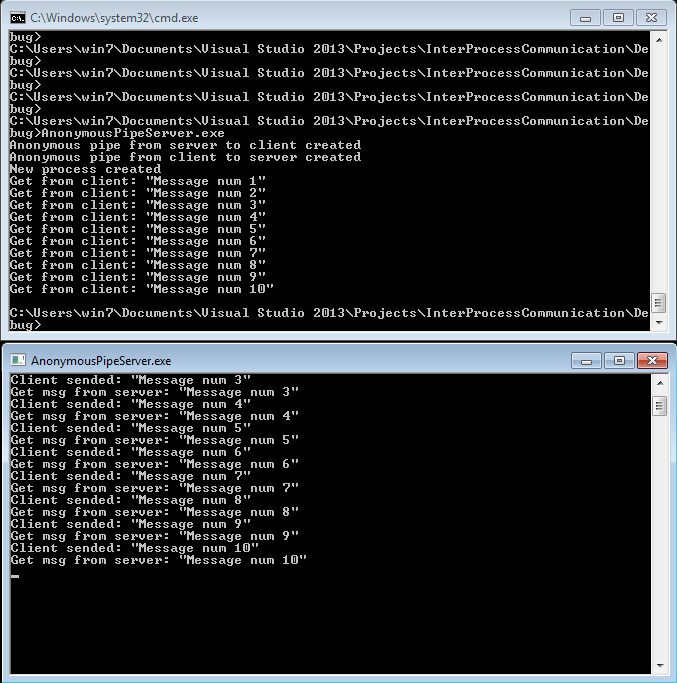
\includegraphics[scale=0.95]{res/02_anonymous_channels}
\caption{Работа с анонимными каналами.}
\end{figure}

Результаты работы показаны на рисунке 2. Листинг 4 и листинг 5 содержат протоколы работы сервера и клиента.

\lstinputlisting[language={},caption={Протокол работы серверного модуля программы работы с анонимными каналами}]{res/AnonymousPipeServer.log}

\lstinputlisting[language={},caption={Протокол работы клиентского модуля программы работы с анонимными каналами}]{res/AnonymousPipeClient.log}

%------------------------------------------------
\chapter*{Именованные каналы}
\addcontentsline{toc}{chapter}{Именованные каналы}

Именованные каналы (named pipes) предлагают ряд возможностей, которые делают их полезными в качестве универсального механизма реализации приложений на основе IPC, включая приложения, требующие сетевого доступа к файлам, и клиент-серверные системы, хотя для реализации простых вариантов IPC, ориентированных на байтовые потоки, как в предыдущем примере, в котором взаимодействие процессов ограничивается рамками одной системы, анонимных каналов вам будет вполне достаточно. К числу упомянутых возможностей (часть которых обеспечивается дополнительно) относятся следующие:

\begin{itemize}
\item Именованные каналы ориентированы на обмен сообщениями, поэтому процесс, выполняющий чтение, может считывать сообщения переменной длины именно в том виде, в каком они были посланы процессом, выполняющим запись.

\item Именованные каналы являются двунаправленными, что позволяет осуществлять обмен сообщениями между двумя процессами посредством единственного канала.

\item Допускается существование нескольких независимых экземпляров канала, имеющих одинаковые имена. Например, с единственной серверной системой могут связываться одновременно несколько клиентов, использующих каналы с одним и тем же именем. Каждый клиент может иметь собственный экземпляр именованного канала, и сервер может использовать этот же канал для отправки ответа клиенту.

\item Каждая из систем, подключенных к сети, может обратиться к каналу, используя его имя. Взаимодействие посредством именованного канала осуществляется одинаковым образом для процессов, выполняющихся как на одной и той же, так и на разных машинах.

\item Имеется несколько вспомогательных и связных функций, упрощающих обслуживание взаимодействия "запрос/ответ" и клиент-серверных соединений.
\end{itemize}

Как правило, именованные каналы являются более предпочтительными по сравнению с анонимными, хотя существуют ситуации, когда анонимные каналы оказываются исключительно полезными. Во всех случаях, когда требуется, чтобы канал связи был двунаправленным, ориентированным на обмен сообщениями или доступным для нескольких клиентских процессов, следует применять именованные каналы.

Реализация работы с именованными каналами представлена в листинге 8 (серверный модуль) и 9 (клиентский модуль). Сервер, как и ранее, создает все необходимые ресурсы и переходит в состояние ожидания соединений. Именованный канал создается для чтения и записи. Передача происходит сообщениями, функции передачи и приема блокируются до их окончания.

\lstinputlisting[language=C++, caption={Клиент именованного каналов}]
{../../src/InterProcessCommunication/NamedPipeClient/main.cpp}
\vspace{3em}

Клиент после соединения с сервером начинает чтение сообщений с консоли, пока не
встретит слово «exit». По данному слову и клиент и сервер завершают свою работу.

Для данной программы были внесены изменения в логер. Теперь каждый клиентский процесс создаёт свой отдельный файл с протоколом.

\lstinputlisting[language=C++, caption={Клиент именованного каналов}]
{../../src/InterProcessCommunication/NamedPipeClient/main.cpp}
\vspace{3em}

Результат работы программы показан на рисунке 3. Запущен один сервер и три клиента, с которыми этот сервер взаимодействует.
\vspace{2em}

\begin{figure}[h!]
\centering
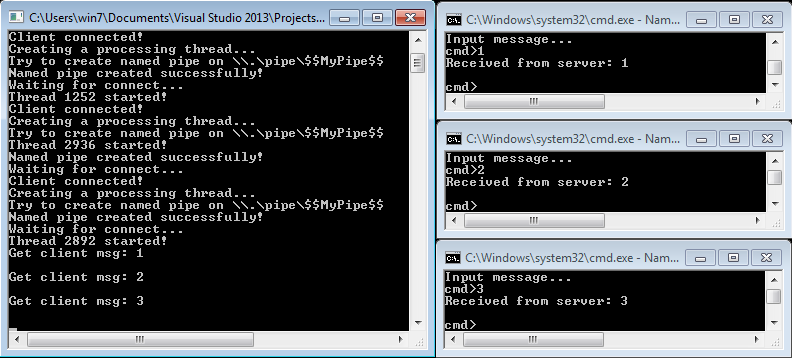
\includegraphics[scale=0.75]{res/03_named_pipes}
\caption{Работа нескольких клиентов с одним сервером по именованному каналу.}
\end{figure}

Программа Process Explorer известного разработчика Марка Русиновича позволяет отследить, кто использует именованные каналы. На рисунке 4 видно, что клиентский модуль использует канал MyPipe.
\vspace{2em}

\begin{figure}[h!]
\centering
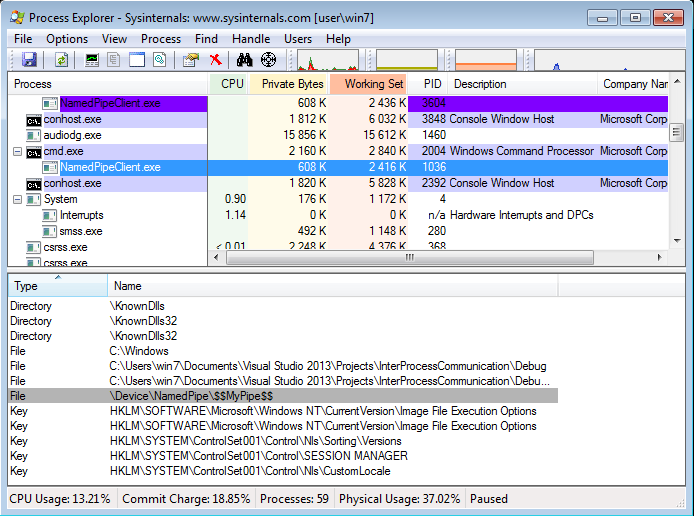
\includegraphics[scale=0.85]{res/04_Process_Explorer_np}
\caption{Отслеживания обращений к локальным (не сетевым) именованным каналам}
\end{figure}

\begin{figure}[h!]
\centering
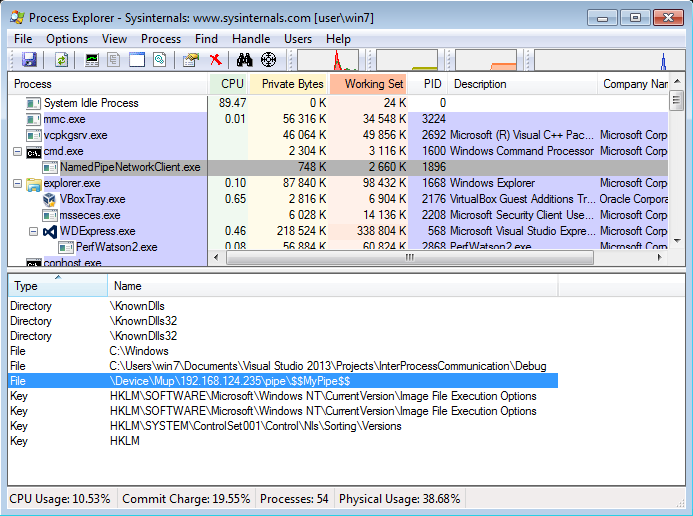
\includegraphics[scale=0.85]{res/05_Process_Explorer_npn}
\caption{Отслеживания обращений к сетевым именованным каналам в Process Explorer}
\end{figure}

Помимо локального обмена, именованные каналы могут использоваться и для сетевого взаимодействия. Это требует не большой доработки клиента в части указания пути к каналу и изменения настроек безопасности: клиент обращается к именованному каналу указывая имя серверного хоста или его IP адрес. Работа сетевой версии программы показана на рисунке 5. 

%------------------------------------------------
\chapter*{Почтовые ящики}
\addcontentsline{toc}{chapter}{Почтовые ящики}

Как и именованные каналы, почтовые ящики (mailslots) Windows снабжаются именами, которые могут быть использованы для обеспечения взаимодействия между независимыми каналами. Почтовые ящики представляют собой широковещательный механизм, и ведут себя иначе по сравнению с именованными каналами, что делает их весьма полезными в ряде ограниченных ситуаций, которые, тем не менее, представляют большой интерес. Из наиболее важных свойств почтовых ящиков можно отметить следующие:

\begin{itemize}
\item Почтовые ящики являются однонаправленными.

\item С одним почтовым ящиком могут быть связаны несколько записывающих программ (writers) и несколько считывающих программ (readers), но они часто связаны между собой отношениями "один ко многим" в той или иной форме.

\item Записывающей программе (клиенту) не известно достоверно, все ли, только некоторые или какая-то одна из программ считывания (сервер) получили сообщение.

\item Почтовые ящики могут находиться в любом месте сети.

\item Размер сообщений ограничен.
\end{itemize}

Использование почтовых ящиков требует выполнения следующих операций:
\begin{itemize}
\item Каждый сервер создает дескриптор почтового ящика с помощью функции CreateMailSlot.

\item После этого сервер ожидает получения почтового сообщения, используя функцию ReadFile.

\item Клиент, обладающий только правами записи, должен открыть почтовый ящик, вызвав функцию CreateFile, и записать сообщения, используя функцию WriteFile. В случае отсутствия ожидающих программ считывания попытка открытия почтового ящика завершится ошибкой (наподобие "имя не найдено").
\end{itemize}

Сообщение клиента может быть прочитано всеми серверами; все серверы получают одно и то же сообщение.

Листинг 8 и 9 демонстрируют реализацию приложения, иллюстрирующую обмен информацией почтовыми слотами. В процессе экспериментов было протестировано локальное, сетевое взаимодействие. Для широковещательной передач сообщений, адрес заменялся символом звездочки (*).

\lstinputlisting[language=C++, caption={Реализация серверной части почтового ящика}]
{../../src/InterProcessCommunication/MailslotServer/main.cpp}

\vspace{3em}

\lstinputlisting[language=C++, caption={Реализация клиентской части почтового ящика}]
{../../src/InterProcessCommunication/MailslotClient/main.cpp}

Результат работы программы показан на рисунке 6.

\begin{figure}[h!]
\centering
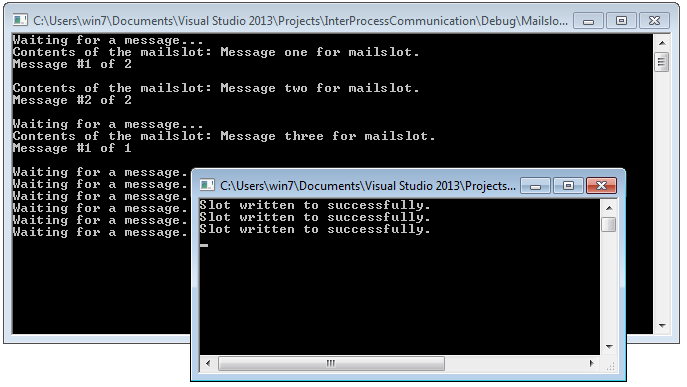
\includegraphics[scale=0.95]{res/06_MailSlot}
\caption{Работа почтовыми ящиками.}
\end{figure}

На рисунке 7 показана работа почтового ящика в Process Explorer. Листинг 10 и 11 содержит протокол работы программы.

\lstinputlisting[language={},caption={Протокол работы серверного модуля программы работы с почтовыми ящиками}]{res/MailslotServer.log}

\lstinputlisting[language={},caption={Протокол работы клиентского модуля программы работы с почтовыми ящиками}]{res/MailslotClient.log}

Существует еще одна возможность. В вызове функции CreateFile клиент может указать имя почтового ящика в следующем виде:

\begin{verbatim}\\*\mailslot\mailslotname
\end{verbatim}

При этом символ звездочки (*) действует в качестве группового символа (wildcard), и клиент может обнаружить любой сервер в пределах имени домена — группы систем, объединенных общим именем, которое назначается администратором сети. 

\begin{figure}[h!]
\centering
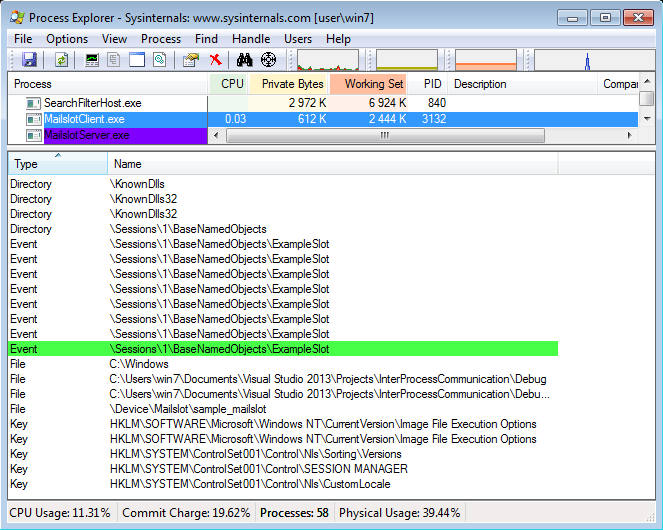
\includegraphics[scale=0.75]{res/07_Process_Explorer}
\caption{Работа почтовыми ящиками.}
\end{figure}


%------------------------------------------------
\chapter*{Shared memory}
\addcontentsline{toc}{chapter}{Shared memory}

Этот способ взаимодействия реализуется через технологию File Mapping - отображения файлов на оперативную память. Механизм позволяет осуществлять доступ к файлу таким образом, как будто это обыкновенный массив, хранящийся в памяти (не загружая файл в память явно). Можно создать объект file mapping, но не ассоциировать его с каким-то конкретным файлом. Получаемая область памяти будет общей между процессами. Работая с этой памятью, потоки обязательно должны согласовывать свои действия с помощью объектов синхронизации.

В листинге 12 и 13 представлен код двух программ, одна из которых генерирует случайные числа, а другая их читает и выводит на экран. Взаимодействие осуществляется через разделяемую память, защищённую мьютексом. Рисунок 8 показывает результат такого взаимодействия.

\lstinputlisting[language=C++, caption={Программа, генерирующая случайные числа в разделяемую память}]
{../../src/InterProcessCommunication/SharedMemoryServer/main.cpp}

\vspace{3em}

\lstinputlisting[language=C++, caption={Программа, читающая случайные числа из разделяемой памяти}]
{../../src/InterProcessCommunication/SharedMemoryClient/main.cpp}

\newpage
\begin{figure}[h!]
\centering
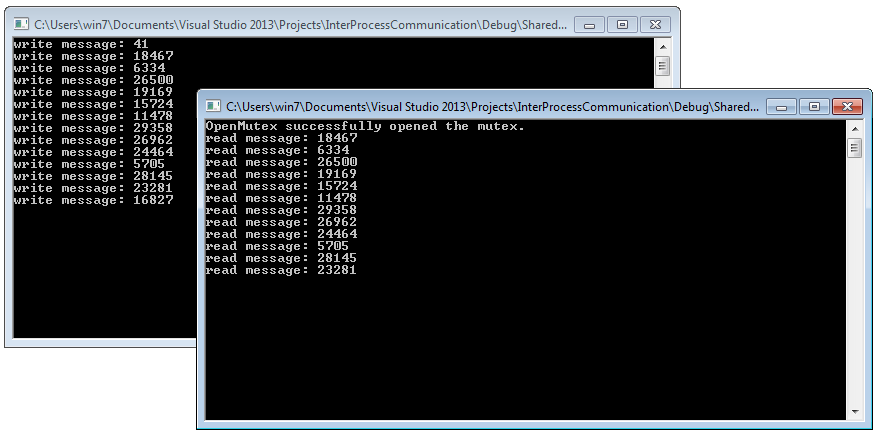
\includegraphics[scale=0.75]{res/08_Sharedmemory}
\caption{Работа с разделяемой памятью.}
\end{figure}

Листинг 14 и 15 содержит протокол (он не много подрезан для краткости) работы программы. Интерес здесь представляет порядок захвата мьютекса.

\lstinputlisting[language={},caption={Протокол работы серверного модуля программы работы с разделяемой памятью}]{res/SharedMemoryServer.log}

\lstinputlisting[language={},caption={Протокол работы клиентского модуля программы работы с разделяемой памятью}]{res/SharedMemoryClient.log}

На рисунке 9 видно, как программа клиент работает с ресурсами. Две последние строчки, это мьютекс и общая память.


\begin{figure}[h!]
\centering
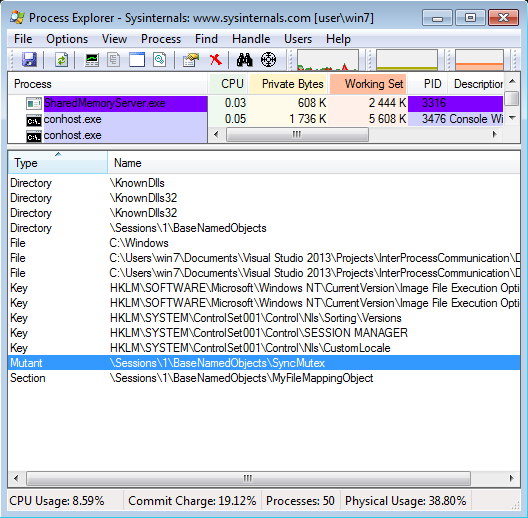
\includegraphics[scale=1]{res/09_Process_Explorer}
\caption{Мьютекс и общая память}
\end{figure}

%------------------------------------------------
\chapter*{Сокеты}
\addcontentsline{toc}{chapter}{Сокеты}

Winsock API разрабатывался как расширение Berkley Sockets API для среды Windows и поэтому поддерживается всеми системами Windows. К особенностям Winsock можно отнести следующее:

\begin{itemize}
\item Перенос уже имеющегося кода, написанного для Berkeley Sockets API, осуществляется непосредственно.

\item Системы Windows легко встраиваются в сети, использующие как версию IPv4 протокола TCP/IP, так и постепенно распространяющуюся версию IPv6. Помимо всего остального, версия IPv6 допускает использование более длинных IP-адресов, преодолевая существующий 4-байтовый адресный барьер версии IPv4.

\item Сокеты могут использоваться совместно с перекрывающимся вводом/выводом Windows, что, помимо всего прочего, обеспечивает возможность масштабирования серверов при увеличении количества активных клиентов.

\item Сокеты можно рассматривать как дескрипторы (типа HANDLE) файлов при использовании функций ReadFile и WriteFile и, с некоторыми ограничениями, при использовании других функций, точно так же, как в качестве дескрипторов файлов сокеты применяются в UNIX. Эта возможность оказывается удобной в тех случаях, когда требуется использование асинхронного ввода/вывода и портов завершения ввода/вывода.

\item Существуют также дополнительные, непереносимые расширения.
\end{itemize}

Работа с сокетами демонстрируется в листинге 16 и 17. Рисунок 6 показывает работу программ, из этих листингов.


\lstinputlisting[language=C++, caption={Сервер для работы с Win-сокетами}]
{../../src/InterProcessCommunication/WinSockServer/main.cpp}

Клиент отправляет серверу сообщения, и получает эхо-ответ. Слово QUIT зарезервировано для завершения работы.

\lstinputlisting[language=C++, caption={Клиент для работы с Win-сокетами}]
{../../src/InterProcessCommunication/WinSockClient/main.cpp}

Листинг 18 и 19 содержит протокол работы программы.

\lstinputlisting[language={},caption={Протокол работы серверного модуля программы работы с сокетами Windows}]{res/WinSockServer.log}

\lstinputlisting[language={},caption={Протокол работы клиентского модуля программы работы с сокетами Windows}]{res/WinSockClient.log}

\begin{figure}[h!]
\centering
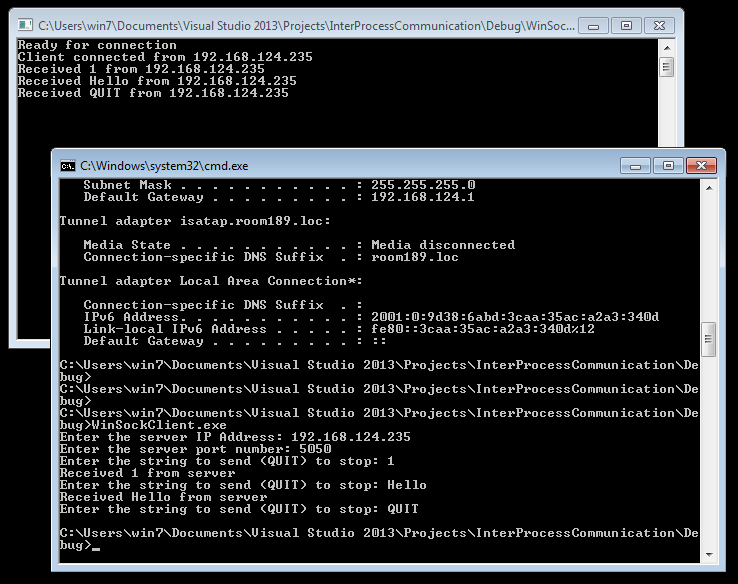
\includegraphics[scale=0.85]{res/10_Winsock}
\caption{Работа с сокетами.}
\end{figure}

Результаты работы программы показаны на рисунке 10. Клиент соединяется с сервером по локальному IP адресу. Серверный слушающий сокет связан с адресом INADDR\_ANY, т.е. прослушивает все сетевые интерфейсы.

\begin{figure}[h!]
\centering
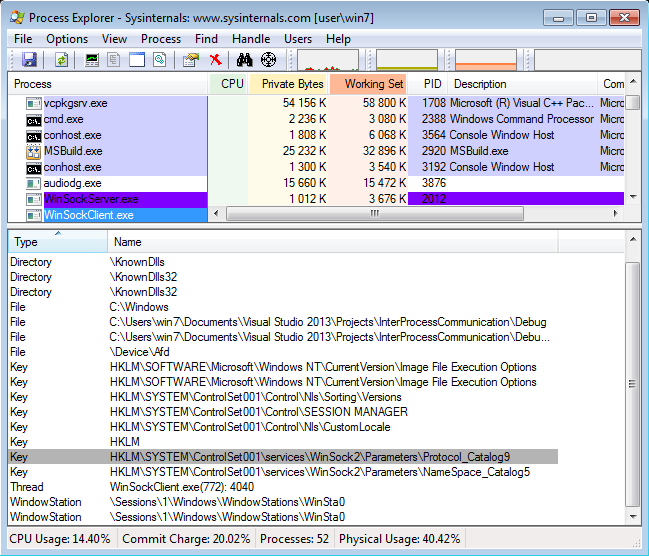
\includegraphics[scale=1]{res/11_Process_Explorer}
\caption{Сокеты в списке ресурсов}
\end{figure}

На рисунке 11 показано как сокеты видны системе.

Библиотека Winsock поддерживает два вида сокетов -- синхронные (блокируемые) и асинхронные (неблокируемые). Синхронные сокеты задерживают управление на время выполнения операции, а асинхронные возвращают его немедленно, продолжая выполнение в фоновом режиме, и, закончив работу, уведомляют об этом вызывающий код.

Сокеты позволяют работать со множеством протоколов и являются удобным средством межпроцессорного взаимодействия, но в данной работе рассматриваются только сокеты семейства протоколов TCP/IP, использующихся для обмена данными между узлами сети Интернет.

Независимо от вида, сокеты делятся на два типа -- потоковые и дейтаграммные. Потоковые сокеты работают с установкой соединения, обеспечивая надежную идентификацию обоих сторон и гарантируют целостность и успешность доставки данных. Дейтаграмные сокеты работают без установки соединения и не обеспечивают ни идентификации отправителя, ни контроля успешности доставки данных, зато они заметно быстрее потоковых. Дейтаграммные сокеты опираются на протокол UDP, а потоковые на TCP.

Выбор того или иного типа сокетов определяется транспортным протоколом, на котором работает сервер, -- клиент не может по своему желанию установить с дейтаграммным сервером потоковое соединение.

%------------------------------------------------
\chapter*{Порты завершения}
\addcontentsline{toc}{chapter}{Порты завершения}

Операциям ввода и вывода присуща более медленная скорость выполнения по сравнению с другими видами обработки. Причиной такого замедления являются следующие факторы:

\begin{itemize}
\item Задержки, обусловленные затратами времени на поиск нужных дорожек и секторов на устройствах произвольного доступа (диски, компакт-диски).

\item Задержки, обусловленные сравнительно низкой скоростью обмена данными между физическими устройствами и системной памятью.

\item Задержки при передаче данных по сети с использованием файловых, серверов, хранилищ данных и так далее.
\end{itemize}

Во всех предыдущих примерах операции ввода/вывода выполняются синхронно с потоком, поэтому весь поток вынужден простаивать, пока они не завершатся.
\vspace{1em}

В этом примере показано, каким образом можно организовать продолжение выполнения потока, не дожидаясь завершения операций ввода/вывода, что будет соответствовать выполнению потоками асинхронного ввода/вывода.
\vspace{1em}

Порты завершения оказываются чрезвычайно полезными при построении масштабируемых серверов, способных обеспечивать поддержку большого количества клиентов без создания для каждого из них отдельного потока. 
\vspace{1em}

Листинг 20 показывает реализацию порта завершения. Для работы с ним использовался клиент из предыдущего примера.

\lstinputlisting[language=C++, caption={Порт завершения}]
{../../src/InterProcessCommunication/CompletionPortServer/main.cpp}

Листинги 21 и 22 содержат протокол работы программы. Стоит обратить внимание, что в отличии от предыдущего примера, когда клиент ожидал данные сразу после отправки, здесь клиент получает ответ асинхронно.

\lstinputlisting[language={},caption={Протокол работы серверного модуля программы работы с портами завершения}]{res/CompletionPortServer.log}

\lstinputlisting[language={},caption={Протокол работы клиентского модуля программы работы с портами завершения}]{res/WinSockClient-comlp.log}

Рисунок 12 показывает работу программы, а на рисунке 13 видны несколько процессов серверного модуля (в клиентском модуле никаких изменений, по сравнению с обычными сокетами нет).

\begin{figure}[h!]
\centering
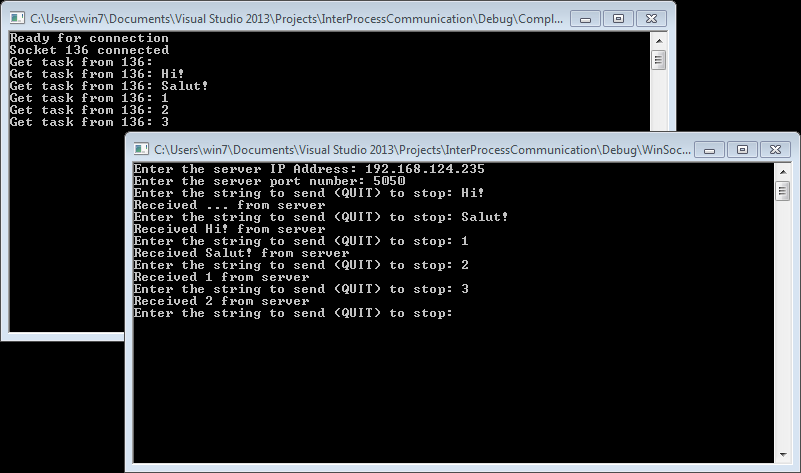
\includegraphics[scale=0.8]{res/12_Completion_Port}
\caption{Программа работы с портами завершения}
\end{figure}

\begin{figure}[h!]
\centering
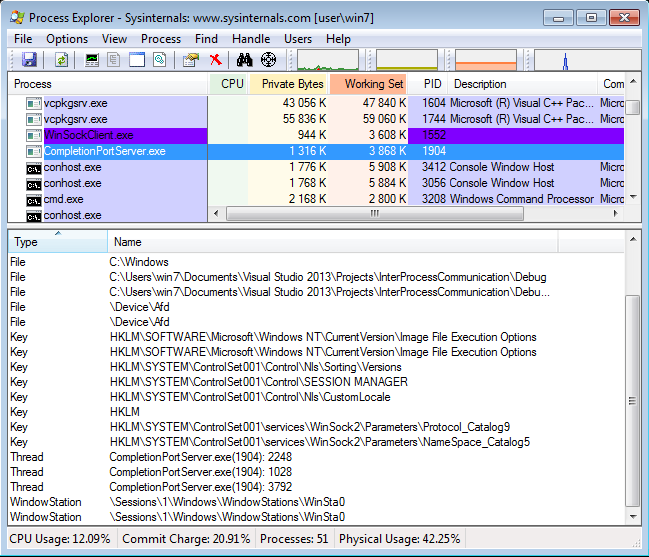
\includegraphics[scale=0.8]{res/13_Process_Explorer}
\caption{Процессы серверного модуля}
\end{figure}

%------------------------------------------------
\chapter*{Сигналы}
\addcontentsline{toc}{chapter}{Сигналы}

В отличии от Linux, сигналы в Windows имеют сильно усеченные возможности. Наиболее сложной задаче при работе с сигналами было придумать, что можно с ними сделать. В листинге 23 по сигналу меняется цвет консоли, это видно на рисунке 14.

\lstinputlisting[language=C++, caption={Сигналы в Windows}]
{../../src/InterProcessCommunication/Signals/main.cpp}
\vspace{1em}

\begin{figure}[h!]
\centering
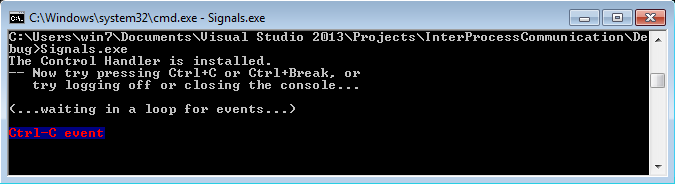
\includegraphics[scale=0.95]{res/14_Signals}
\caption{Работа с сигналами в Windows}
\end{figure}

%------------------------------------------------
\chapter*{Заключение}
\addcontentsline{toc}{chapter}{Заключение}

В данной работе были рассмотрены основные механизмы межпроцессорного взаимодействия, от самых простых, типа анонимных каналов, до самых сложных, таких как сокеты и порты завершения. Каждый механизм имеет свою нишу для использования.
\vspace{1em}

Отдельно выделяются только сигналы, которые значительно уступают подобному механизму из мира linux.
\vspace{1em}

Наиболее интересным средством взаимодействия оказался сокет. Он не имеет больших отличий от классического сокета Беркли, что упрощает его изучение. Работа в асинхронном режиме (порты завершения) оказывает драматическое влияние на скорость работы системы, и должна применяться в высоко нагруженных системах.

\end{document}
